%Resistors_Capacitors
\chapter{Resistors and Capacitors}
In this lab, we will not build a new instrument. We will use an instrument we built in a previous lab (or at least only a new version of that instrument adjusted for today's resistance values). You will notice a pattern in what we do from now on in PH250. We will build an instrument and then test a model with that instrument. The instrument must be designed so that it can take the data needed to test the model. In today's lab, we will test the model of how capacitors work in a circuit. If your PH220 class is
moving along nicely, this model will be familiar.

\section{The Model to Test}

\begin{figure}[h!]
	\centering
	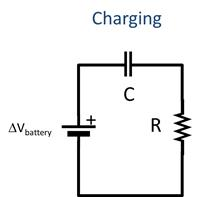
\includegraphics[width=1.67in,height=1.67in]{PH4CAW37}
\end{figure}

Let's start by thinking of hooking up a capacitor and a resistor in series with a battery. The capacitor will become charged. The voltage across the capacitor as a function of time will be given by

\begin{equation*}
	\Delta V_{C}\left( t\right) =\Delta V_{\max }\left( 1-e^{-\frac{t}{\tau } }\right) \qquad \text{Charging}
	\label{charging}
\end{equation*}

\noindent where 

\begin{equation}
	\tau =RC
\end{equation}

\noindent is the product of the resistance, $R$, and the capacitance, $C.$ The current in the circuit as a function of time will be given by 

\begin{equation*}
	I\left( t\right) =I_{\max }e^{-\frac{t}{\tau }}\qquad \text{Charging}
\end{equation*}

\noindent while we charge up the capacitor. The quantity 

\begin{equation*}
	\tau =RC
\end{equation*}

\noindent is called the time constant.

We should review what a time constant is. Think of a particular case, say, 

\begin{eqnarray*}
	\Delta V_{battery} &=&1.5\unit{V} \\R &=&2\unit{\Omega} \\C &=&10\unit{F}
\end{eqnarray*}

\noindent then

\begin{equation*}
	V_{C}(t)=\left( 1.5\unit{V}\right) \left( 1-e^{-\frac{t}{\left( 2\unit{\Omega}\right) \left( 10\unit{F}\right) }}\right)
\end{equation*}

\noindent and 

\begin{eqnarray*}
	\tau &=&\left( 2\unit{\Omega}\right) \left( 10\unit{F}\right) \\
	     &=&\allowbreak 20.0\unit{s}
\end{eqnarray*}

We can plot this
\begin{figure}[h!]
	\centering
	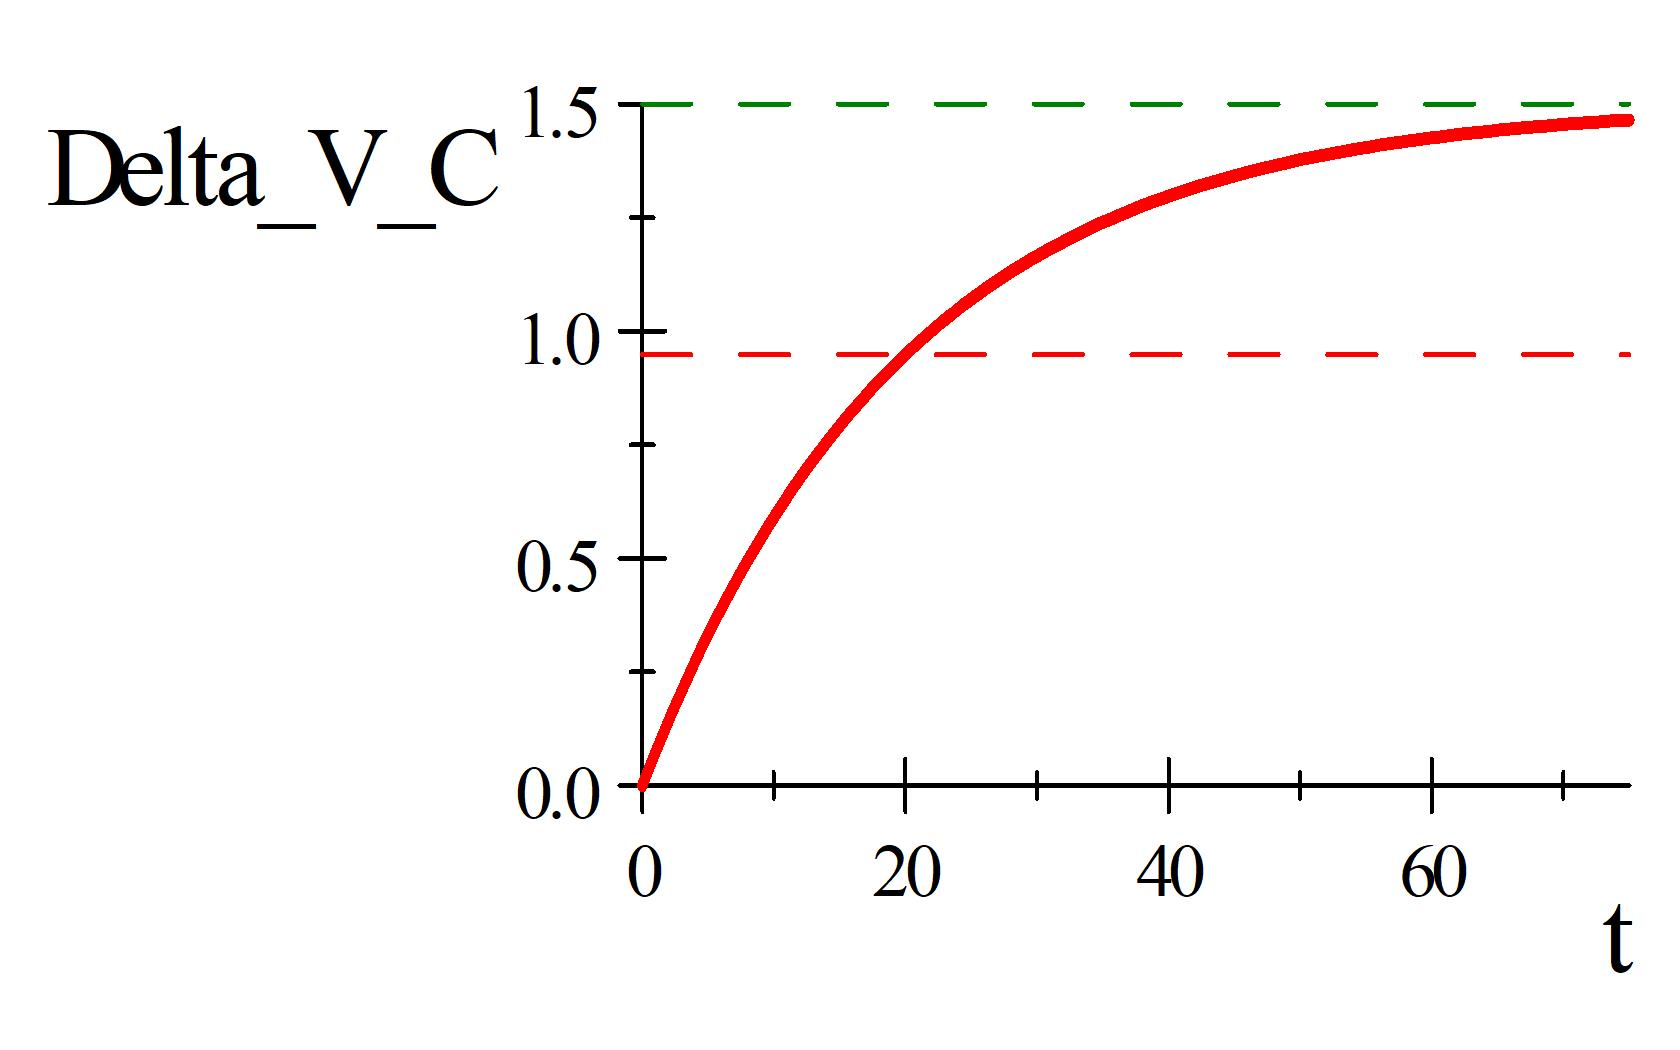
\includegraphics[width=2.8885in,height=1.58in]{PH4CAW38}
\end{figure}

Notice, that by about $t=70\unit{s}$ we essentially have $\Delta V_{C}=\Delta V_{battery}.$ But up to that point, the voltage across the capacitor changes in a very non-linear way. The part of the equation that looks like

\begin{equation*}
	\left( 1-e^{-\frac{t}{RC}}\right)
\end{equation*}

\noindent is interesting. What is $e^{0}$?

\begin{equation*}
	e^{0}=1
\end{equation*}

So at $t=0$ we do have $\Delta V_{C}=0$ on the capacitor because 

\begin{equation*}
	\left( 1-e^{-\frac{t}{RC}}\right) =\left( 1-1\right)
\end{equation*}

For any positive time, $e^{-\frac{t}{RC}}$ will be less than $1.$ For large positive times $\frac{t}{RC}$ gets to be a big number. So $e^{-\frac{t}{RC}}$ gets very small. Then  $\left(1-e^{-\frac{t}{RC}}\right) $ gets very close to $1.$ That means that 

\begin{equation*}
	\underset{t\rightarrow \infty }{\lim }\Delta V_{C}=\underset{t\rightarrow\infty }{\lim }\Delta V_{battery}\left( 1-e^{-\frac{t}{RC}}\right) =\Delta V_{battery}\left( 1\right) =\Delta V_{battery}
\end{equation*}

\noindent just as we saw in the graph and as we know it must.

But what if $t=\tau =RC?$ Then 

\begin{eqnarray*}
	\Delta V_{C} &=&\Delta V_{battery}\left( 1-e^{-\frac{RC}{RC}}\right) = \\
	             &=&\Delta V_{battery}\left( 1-e^{-1}\right) \\
	             &=&\allowbreak 0.632\,12\Delta V_{battery} \\
	             &\approx &63\%\Delta V_{battery}
\end{eqnarray*}

The time $\tau $ is the time it takes for the capacitor to be $63\%$ charged!

The quantity $\tau $ is called the \emph{time constant} because it tells us something about how long it takes for $\Delta V_{c}$ to go from $0$ to get to $\Delta V_{battery}.$ The ``t-looking-thing'' is a Greek letter ``t.'' It is pronounced ``tau.'' This quantity will be useful in planning your experiment.

Notice what we have done. We have used our model to form an equation, and we have used part of that equation to understand how much time it will take to perform a test (experiment) of the model. This is typical, get an idea of how to make the measurement from the model we are testing.

But! you say, I don't really remember where all of these equations came from. Or maybe your PH220 class hasn't gotten to allowing current to flow yet so you have not done this. If any of this is mysterious, please read the section of our PH220 book that covers RC circuits. But if it is vaguely familiar or seems to make sense, really we can test our model of how capacitors work just knowing a little about capacitors and the equations that came from the model.

\section{The Instrument}

To test our capacitor model we need to measure the voltage across the capacitor as a function of time. We could also measure the current in the circuit as a function of time. One of these is sufficient to test the model. I am going to describe measuring the voltage across the capacitor as a function of time. But you know from a previous lab how we might add current as a function of time.

We need a device that measures voltage and how it changes as a function of time. But that is just what our Arduino's do! We already know how to build this device. Suppose we can live with a $0\unit{V}$ to $+5\unit{V}$ range of $\Delta V_{battery}.$ Then even our simple voltmeter will work. Since it is a function of time that we are testing, we need to output both voltage and time from our Arduino. We can't guarantee that either of our capacitor leads will be at ground, so we will have to be careful in wiring this voltmeter to give $\Delta V_{C}.$

Remember that $\Delta V_{C}$ is the difference between two voltage
measurements. 

\begin{figure}[h!]
	\centering
	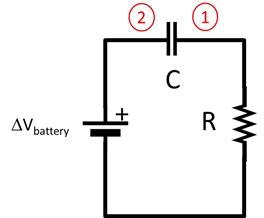
\includegraphics[width=2.2321in,height=1.8455in]{PH4CAW39}
\end{figure}

\noindent so 

\begin{equation*}
	\Delta V_{C}=V_{2}-V_{1}
\end{equation*}

neither of which will be ground, so we really have to measure both with our Arduino. We also need a ground connection. The wiring diagram might look like this:

\begin{figure}[h!]
	\centering
	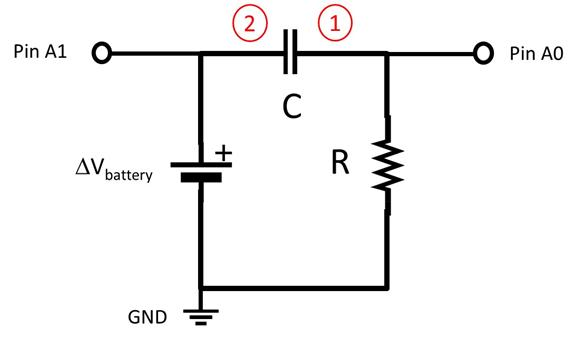
\includegraphics[width=3.2759in,height=1.9501in]{PH4CAW3A}
\end{figure}

\noindent and our sketch will be a little like the one from our last lab.

\vspace{0.24in}
%%%%%%%%%%%%%%%%%%%%%%%%%%%%%%%%%%%%%%%%%%%%%%%%%%%%%%%%%%%%%%%%%%%%
\href{https://raw.githubusercontent.com/rtlines/IntermediateLabPH250/main/Code/RC_Volts_vsTime.ino}{Download here}
%%%%%%%%%%%%%%%%%%%%%%%%%%%%%%%%%%%%%%%%%%%%%%%%%%%%%%%%%%%%%%%%%%%%
\lstinputlisting[language=Arduino]{Code/RC_Volts_vsTime.ino}

This is just a voltmeter, but one with two A2D pins and a ground. This sketch also gives us time using the millis() function. This function gives the number of milliseconds since our experiment began. We can use our python code from a previous lab to save the data into a file. I modified the previous code just a bit, so here is an updated version.

%%%%%%%%%%%%%%%%%%%%%%%%%%%%%%%%%%%%%%%%%%%%%%%%%%%%%%%%%%%%%%%%%%%%
\href{https://raw.githubusercontent.com/rtlines/IntermediateLabPH250/main/Code/RC_ReadSaveFile.py}{Download here}
%%%%%%%%%%%%%%%%%%%%%%%%%%%%%%%%%%%%%%%%%%%%%%%%%%%%%%%%%%%%%%%%%%%%
\inputpython{Code/RC_ReadSaveFile.py}{0}{10000}

The resulting data could be plotted in python. It might look something like this.

\begin{figure}[h!]
	\centering
	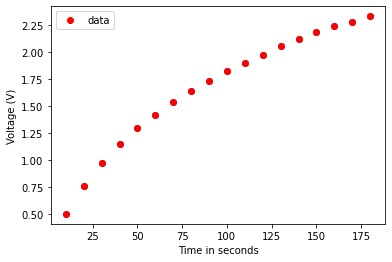
\includegraphics[width=2.9101in,height=1.7538in]{RC_circuit_data}
\end{figure}

I plotted this in python. You might plot it in Excel or LoggerPro  or many other plotting tools. Before we fit a line to data. But looking at the data, a linear fit doesn't seem appropriate for this data. So we need to go beyond what we have done so far. To do this we need a curve fit tool that can use whatever equation that might fit the data. Python can do this, and so can LoggerPro.  But Excel can't. We will have to be more picky about what tool to use to match our data. 

%%%%%%%%%%%%%%%%%%%%%%%%%%%%%%%%%%%%%%%%%%%%%%%%%%%%%%%%%%%%%%%%%%%%
% include a module on curve fitting for non-linear functions. As of this writing 
%   the choices are using 
%%%%%%%%%%%%%%%%%%%%%%%%%%%%%%%%%%%%%%%%%%%%%%%%%%%%%%%%%%%%%%%%%%%%
%	\subsection{LoggerPro Curve Fitting.}

Let's start by noting that you can download LoggerPro to your own computer
if you would like. You should have received a notification about this on
I-Learn. If you wish to install LoggerPro, follow the announcement
instructions.

Once you have LoggerPro on your computer or on one of our lab computers, we
will use it for fitting a curve to our data just like we did last time in
Excel. Suppose you have already imported your data in Excel. It might look
like this:

\begin{figure}[h!]
	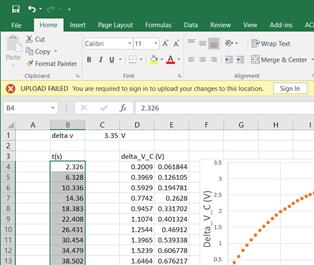
\includegraphics[width=2.6498in,height=2.2399in]{PH4CAX3C}
\end{figure}Now highlight a----- column (I
highlighted the time column) and select copy to copy the data to the
clipboard. Then open up LoggerPro. You will see a data area, a graph area,
and the toolbar.\begin{figure}[h!]
	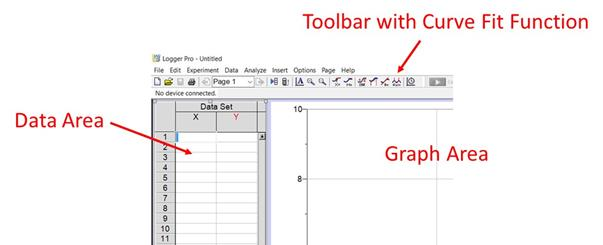
\includegraphics[width=5.0721in,height=2.0721in]{PH4CAX3D}
\end{figure}We want to past the data into a
column in LoggerPro. If you also selected the time data, paste it into the $%
x $-column in Logger Pro. \begin{figure}[h!]
	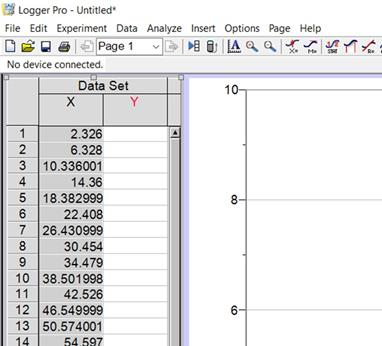
\includegraphics[width=3.2197in,height=2.9187in]{PH4CAX3E}
\end{figure}

Do the same for the voltage data. Paste it into the $y$-column. Once you do
this, the data will automatically be graphed. \begin{figure}[h!]
	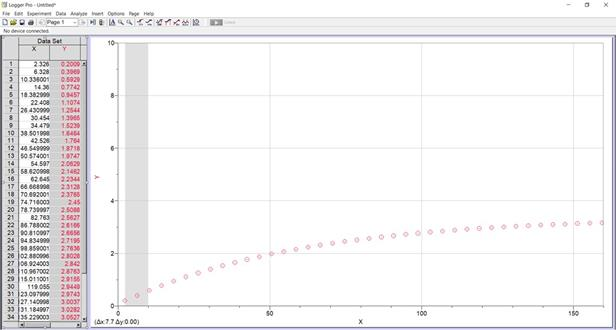
\includegraphics[width=5.1802in,height=%
	2.7838in]{PH4CAX3F}
\end{figure}We now want to fit a curve to
this data. The curve fit function can be accessed from the tool bar. It
looks like this: \begin{figure}[h!]
	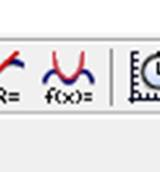
\includegraphics[width=1.3604in,height=1.4607in]{PH4CAX3G}
\end{figure}Click on the icon and a new
dialog will appear. \begin{figure}[h!]
	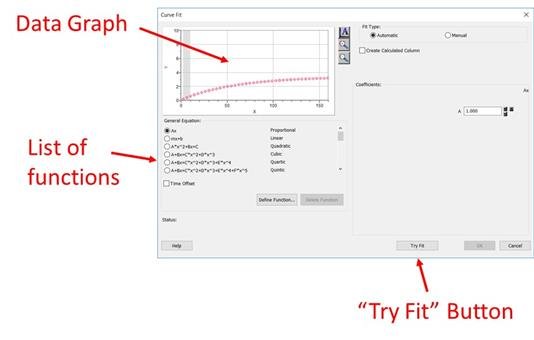
\includegraphics[width=4.4936in,height=2.8677in]{PH4CAX3H}
\end{figure}

It is tempting to try just any function to see if it fits. But the goal is
not to have a great fit. The goal is to see if our data fit the equation
from our capacitor model. 
\begin{equation*}
	\Delta V_{C}\left( t\right) =\Delta V_{\max }\left( 1-e^{-\frac{t}{\tau }%
	}\right)
\end{equation*}%
so we need to find this particular function. This is why I didn't suggest
using Excel. Excel does not have the equation we need in it's list.

\begin{figure}[h!]
	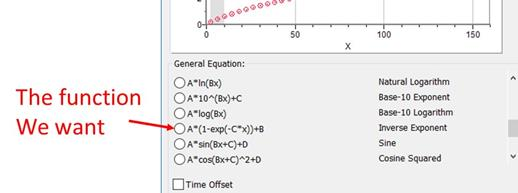
\includegraphics[width=3.2759in,height=1.2298in]{PH4CAX3I}
\end{figure}Of course we won't find a match
with our exact notation. The one we want is given as 
\begin{equation*}
	y=A\ast (1-\exp (-C\ast x))+B
\end{equation*}%
and now we have to match our variables with theirs. Let's compare the
equations. 
\begin{eqnarray*}
	y &=&A\ast (1-\exp (-C\ast x))+B \\
	\Delta V_{C}\left( t\right) &=&\Delta V_{\max }\left( 1-e^{-\frac{t}{\tau }%
	}\right) +0
\end{eqnarray*}%
We can see that 
\begin{equation*}
	\begin{tabular}{ll}
		Ours & Theirs \\ 
		$\Delta V_{\max }$ & $A$ \\ 
		$0$ & $B$ \\ 
		$\tau $ & $\frac{1}{\mathtt{C}}$%
	\end{tabular}%
\end{equation*}%
We can see this \begin{figure}[h!]
	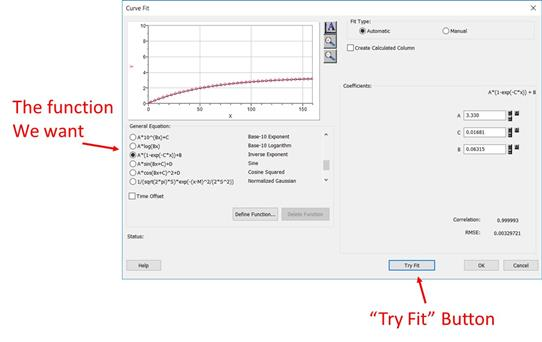
\includegraphics[width=4.561in,height=2.8842in]{PH4CAX3J}
\end{figure}

If the fit looks good, choose the \textquotedblleft OK\textquotedblright\
button. You get the graph back with the curve fit and a new little box. 
\begin{figure}[h!]
	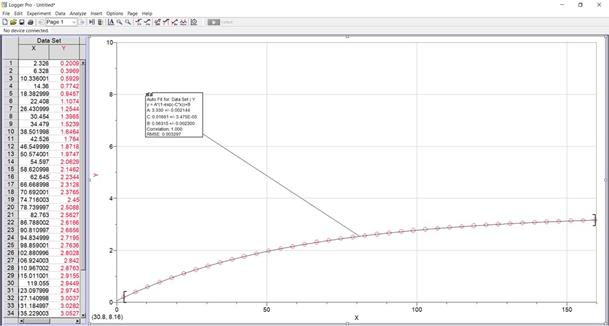
\includegraphics[width=5.1214in,height=2.751in]{PH4CAX3K}
\end{figure}The curve fit looks nice and that
is comforting. For my data, it looks like our capacitor model might be
correct, but we can't be sure until we add in error bars. Before we do that,
let's look at the new little box. \begin{figure}[h!]
	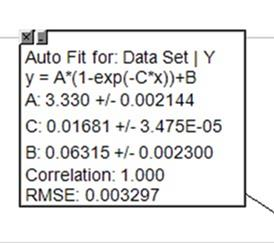
\includegraphics[width=2.3151in,height=2.0557in]{PH4CAX3L}
\end{figure}The box has our fit equation that
we chose and it has values for the fit parameters and their uncertainties.
We will need those later!

Let's add on the error bars now. Right click on the graph if you have a PC
or do the Mac equivalent if you have a Mac. A new dialog appears and in this
case choose \textquotedblleft Graph Options.\textquotedblright\ \begin{figure}[h!]
	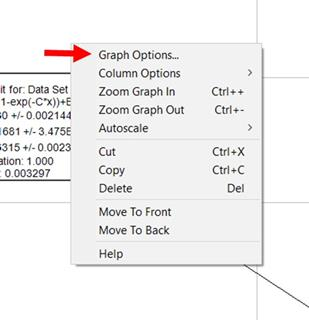
\includegraphics[width=2.6083in,height=2.7008in]{PH4CAX3M}
\end{figure}%
On the \textquotedblleft Graph Options\textquotedblright\ dialog make sure
both $x$ and $y$-error bars are checked.

\begin{figure}[h!]
	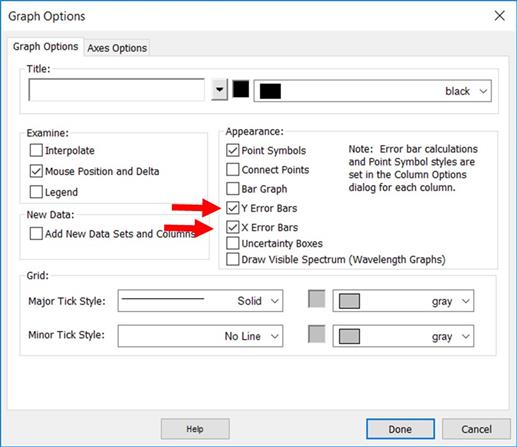
\includegraphics[width=4.3509in,height=3.7645in]{PH4CAX3N}
\end{figure}Chose \textquotedblleft
Done\textquotedblright\ and right click on the graph again. This time choose
\textquotedblleft Column Options.\textquotedblright\ \begin{figure}[h!]
	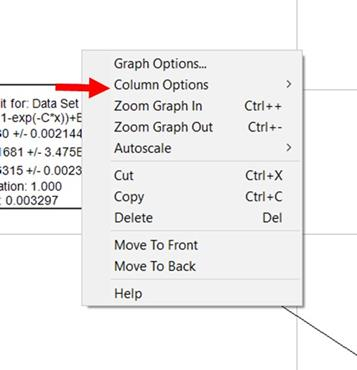
\includegraphics[width=3.0104in,height=%
	3.1185in]{PH4CAX3O}
\end{figure}and choose the $y$-data set.
Another dialog appears with two tabs. Choose the \textquotedblleft
Options\textquotedblright\ tab. \begin{figure}[h!]
	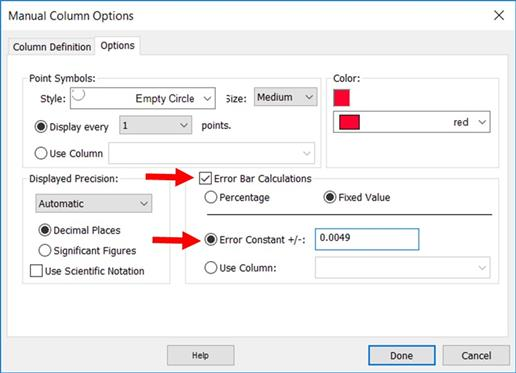
\includegraphics[width=4.3431in,height=3.1453in]{PH4CAX3P}
\end{figure}

You will see a place to choose how error bars are calculated. If you used
the simple voltmeter sketch as your basis, you know the quantization error
is about $4.9\unit{mV}.$ That will be true for every voltage measurement so
we can input this as a constant value. If you used a voltage divider, you
will have to use your calculated error value here. When you have your error
value in place, choose \textquotedblleft Done.\textquotedblright\ \begin{figure}[h!]
	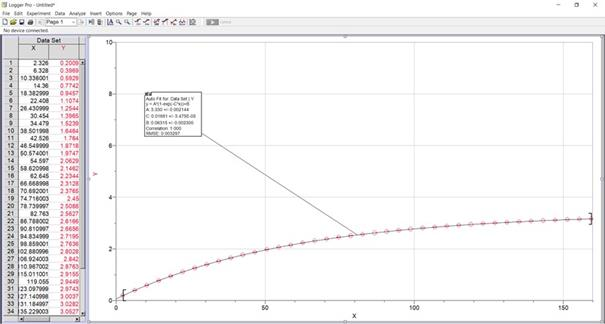
\includegraphics[width=5.0886in,height=2.7345in]{PH4CAX3Q}
\end{figure}

The voltage error was so small that it is hard to see the error bars! That
is fine. What this tells us is that our fit line must go right through the
center of each data point. But it does. So we are really doing fine. The
data supports the model.

But now let's go back to our little box of curve fit parameters. We
identified 
\begin{equation*}
	\tau =\frac{1}{\mathtt{C}}
\end{equation*}%
and for my data I have 
\begin{equation*}
	\mathtt{C}=0.01681\pm 3.475\times 10^{-5}
\end{equation*}%
\newline
We need units, and looking at the equation we know $\tau $ has units of
seconds, so $\mathtt{C}$ must have units of inverse seconds.%
\begin{equation*}
	\mathtt{C}=\left( 0.01681\pm 3.475\times 10^{-5}\right) \frac{1}{\unit{s}}
\end{equation*}%
so we can find a value for $\tau .$ For my data, I have 
\begin{eqnarray*}
	\tau _{measured} &=&\frac{1}{0.01681\frac{1}{\unit{s}}} \\
	&=&59.\,\allowbreak 488\unit{s}
\end{eqnarray*}

Note that we will have to calculate the uncertainty in $\tau .$ I will leave
that for an exercise. But I can compare this $\tau _{measured}$ to the $\tau
=RC$ value I started with. If they are within each other's error range, this
is a powerful confirmation of our capacitor model.

%TCIMACRO{\TeXButton{\vspace*{\fill}}{\vspace*{\fill}}}%
%BeginExpansion
\vspace*{\fill}%
%EndExpansion
\pagebreak
%   or python
%%%%%%%%%%%%%%%%%%%%%%%%%%%%%%%%%%%%%%%%%%%%%%%%%%%%%%%%%%%%%%%%%%%%
\subsection{Python Advanced Curve Fitting.}

In a previous lab we fit a line to a set of data in python. That wasn't very hard. But looking at the sample data in the previous graph, it is clear that a straight line won't do.  The data has a definite curve to it. So what equation do we use for our fit? The only equation that makes sense is the equation we developed from our reasoning about RC circuits.

\begin{equation*}
	\Delta V_{C}\left( t\right) =\Delta V_{\max }\left( 1-e^{-\frac{t}{\tau }}\right) \qquad \text{charging}
\end{equation*}

We can use a different python routine to find a curvy equation like this.  We will use the scipy optimize curve\_fit() routine. But we can help the curve\_fit() routine a little by adding in an extra part. Let's code our fit equation like this

\begin{equation*}
	y=A\ast (1-\exp (-B\ast x))+C
\end{equation*}

where we have added a constant $C$. Of course $C$ should be equal to zero or at least should be close to zero because there is no constant term in our theoretical equation. We will need to check for this in our curve fit solution. 

\href{https://raw.githubusercontent.com/rtlines/IntermediateLabPH250/main/Code/user_function_curve_fit_2.py}{Download here}

\lstinputlisting[language=Arduino]{Code/user_function_curve_fit_2.py}

We have to match our variables with the ones we have in our theory equation. Let's compare the equations. 

\begin{eqnarray*}
	y &=&A\ast (1-\exp (-C\ast x))+B \\
	\Delta V_{C}\left( t\right) &=&\Delta V_{\max }\left( 1-e^{-\frac{t}{\tau }}\right) +0
\end{eqnarray*}

We can see that 

\begin{equation*}
	\begin{tabular}{ll}
	                Theory & python \\ 
		$\Delta V_{\max }$ & $A$ \\ 
	                   $0$ & $B$ \\ 
	               $\tau $ & $\frac{1}{\mathtt{C}}$%
	\end{tabular}
\end{equation*}

I suppose we could have just used the theory variables like $\Delta V_max$ in python. you might choose to do that.

\vspace{1in}

Our curve fit might look like this

\begin{figure}[h!]
	\centering
	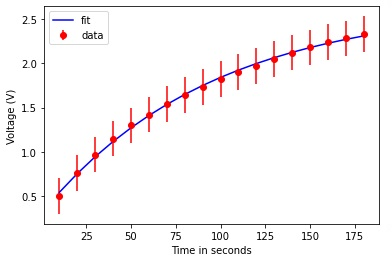
\includegraphics[width=4.561in,height=2.8842in]{RC_circuit_data_with_fit}
\end{figure}

\noindent The program output looks like this:

\begin{verbatim}
	Find a curve fit to a user defined function
	
	The value of A is 2.35419 with standard error of 0.03356.
	The value of B is 0.01051 with standard error of 0.00047.
	The value of C is 0.30913 with standard error of 0.02340.
	
	successful end of program, warning about overflow may follow
\end{verbatim}

If you look at the code you will notice that there is a big difference between the linregress() function and our curve\_fit() function when it comes to the uncertainties in the coefficients. The linregress() function just gave the uncertainteis. But the curve\_fit() function returns a covariance matrix. The diagonal elements of this matrix are our uncertainties on our coefficents -- squared! So we had to take a square root to get the uncertainties.

The curve fit looks nice and that is comforting. For my data, it looks like our capacitor model might be correct, an important thing to check is to see if the curve fit goes through the error bars on all of the data. If it does, it is a good sign that the curve fit might represent the data well.

But now let's go back to our little list of curve fit parameters. We identified 

\begin{equation*}
	\tau =\frac{1}{\mathtt{B}}
\end{equation*}

\noindent and for my data I have 

\begin{equation*}
	\mathtt{B}=0.01051\pm 0.00047
\end{equation*}
\newline

We need units, and looking at the equation we know $\tau $ has units of seconds, so $\mathtt{B}$ must have units of inverse seconds.

\begin{equation*}
	\mathtt{B}=\left( 0.01051\pm 0.00047\right) \frac{1}{\unit{s}}
\end{equation*}

\noindent so we can find a value for $\tau .$ For my data, I have 

\begin{eqnarray*}
	\tau _{measured} &=&\frac{1}{ 0.01051\frac{1}{\unit{s}}} \\
	&=&95.15\,\allowbreak 488\unit{s}
\end{eqnarray*}

Note that we will have to calculate the uncertainty in $\tau .$ I will leave that for an exercise. But I can compare this $\tau _{measured}$ to the $\tau=RC$ value I started with. If they are within each other's error range, this is a powerful confirmation of our capacitor model.



	
\vspace*{\fill}
\pagebreak

\section{Lab Assignment}

We have two equations for charge as a function of time for a RC circuit. They are

\begin{equation*}
	\Delta V_{C}\left( t\right) =\Delta V_{\max }\left( 1-e^{-\frac{t}{\tau }}\right) \qquad \text{charging}
\end{equation*}

\begin{equation*}
	I\left( t\right) =I_{\max }e^{-\frac{t}{\tau }}\qquad \text{charging}
\end{equation*}

\noindent where 

\begin{equation}
	\tau =RC
\end{equation}

\noindent is the time constant.

\begin{enumerate}
	\item 	Using a capacitor with a capacitance of about end $20\unit{\mu F}$ and a resistor of about $1\unit{M\Omega},$ create a circuit as shown. This will be our system that we will use to test our capacitor model.
	
	\begin{figure}[h!]
		\centering
		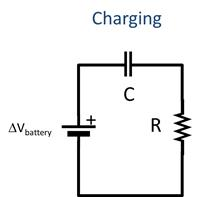
\includegraphics[width=1.67in,height=1.67in]{PH4CAX3R}
	\end{figure}

	You can use one of our power supplies, but be careful to either stay in the $0\unit{V}$ to $+5\unit{V}$ range, or to use a voltage divider to achieve this range at the Arduino input. Follow good lab notebook procedures by recording the model you are testing and your test setup in your lab notebook. Just a note, we will be using directional capacitors. You haven't studied directional capacitors in class. For today's lab, the only difference is that these capacitors only work one direction. This is a little like our diodes. If the circuit doesn't work, try turning your capacitor around.

	\item Build your instrument. and write the sketch and Python collection codes. Test every part of the instrument before you start collecting capacitor data. Don't forget to find your uncertainties. Follow good lab notebook procedures by recording your instrument design in your lab notebook.

	\item Now get ready to collect data for a capacitor charge. Work with a lab partner from your group to achieve the data collection. Compare your data among your group to make sure things went well. Follow good lab notebook procedures by recording your data or giving a location of the stored data in your lab notebook. 
	
	\item Take the data from your file and graph it. Graphing is easy in python, but you could use LoggerPro if you have this on your computer. You should include this graph in your lab notebook (but might also include the curve fit described in  next item on the same graph).

	\item Perform the curve fit. As in the last lab, having the proper curve fit the data is a validation of our model! So if the theoretical curve fits the data, it makes sense that something about the model might be right. Note that we have an equation from our theory, equation (\ref{charging}). If our data fits a different curve, that could be evidence that our theory is wrong! We hope the data fits this curve and no other. But Excel doesn't have this equation built into it. So we can't use Excel this time.  Python might be a good choice, or LoggerPro.  Once you have the curve fit and the fit parameters (and their uncertainties) make a graph of the data and the fit. Error bars would be a good idea. Include the graph of the curve fit and the data in your lab notebook as well as the fit equation and fit parameters (don't forget their uncertainties).

	\item Find the time constant and compare to your predicted value. If these compare within their uncertainties, we have a further validation of the model. Record the time constants and their uncertainties in your lab notebook.

	\item Draw a conclusion, is our capacitor model good?
\end{enumerate}


\vspace*{\fill}
